
\noindent\begin{minipage}{\textwidth}
    \begin{table}[H]
        \centering
        \caption{Hiperparâmetros e Resultados do Melhor Modelo - vit\_v1\_AB\_opt\_aug}
        \vspace{0.2cm}
        \resizebox{\textwidth}{!}{%
            \begin{tabular}{ll | lrrr}
                \hline
                \multicolumn{2}{c|}{\textbf{Hiperparâmetros}} & \multicolumn{4}{c}{\textbf{Métricas por Classe}} \\ \hline
                \textbf{Parâmetro} & \textbf{Valor} & \textbf{Classe} & \textbf{Precisão} & \textbf{Recall} & \textbf{F1-Score} \\ \hline
    Agendador (\$T\_0\$) & 9 & 31.2 & 0.6091 & 0.5929 & 0.6009 \\ 
Agendador de LR & CosineAnnealingWarmRestarts & 31.3 & 0.4261 & 0.4851 & 0.4537 \\ 
Architecture & vit\_b\_16 & 31.4 & 0.4184 & 0.3905 & 0.4039 \\ 
Augmentation (Método) & None & 32.3 & 0.6313 & 0.5765 & 0.6027 \\ 
Batch Size & 32 & 32.4 & 0.3462 & 0.3103 & 0.3273 \\ 
Decaimento de Peso (WD) & 0.0287 & 33.3 & 0.4175 & 0.6425 & 0.5061 \\ 
Dropout & 0.0775 & 41.4 & 0.4211 & 0.1818 & 0.2540 \\ 
Função de Perda & CrossEntropyLoss & 41.5 & 0.5667 & 0.4359 & 0.4928 \\ 
Hidden Units & 256 & 42.4 & 0.7727 & 0.2500 & 0.3778 \\ 
Label Smoothing & 0.0556 & 44.4 & 0.7000 & 0.4828 & 0.5714 \\ 
\cline{3-6} 
Otimizador & AdamW & \textbf{Média (Macro)} & 0.5345 & 0.4591 & 0.4796 \\ 
Taxa de Aprendizado (LR) & 2.23e-05 & \textbf{MCC} & \multicolumn{3}{c}{0.4185} \\ 
Unfreeze Layers & 4 &  & & &  \\ 
            \hline
            \end{tabular}%
        }
    \end{table}

    \begin{figure}[H]
        \centering
        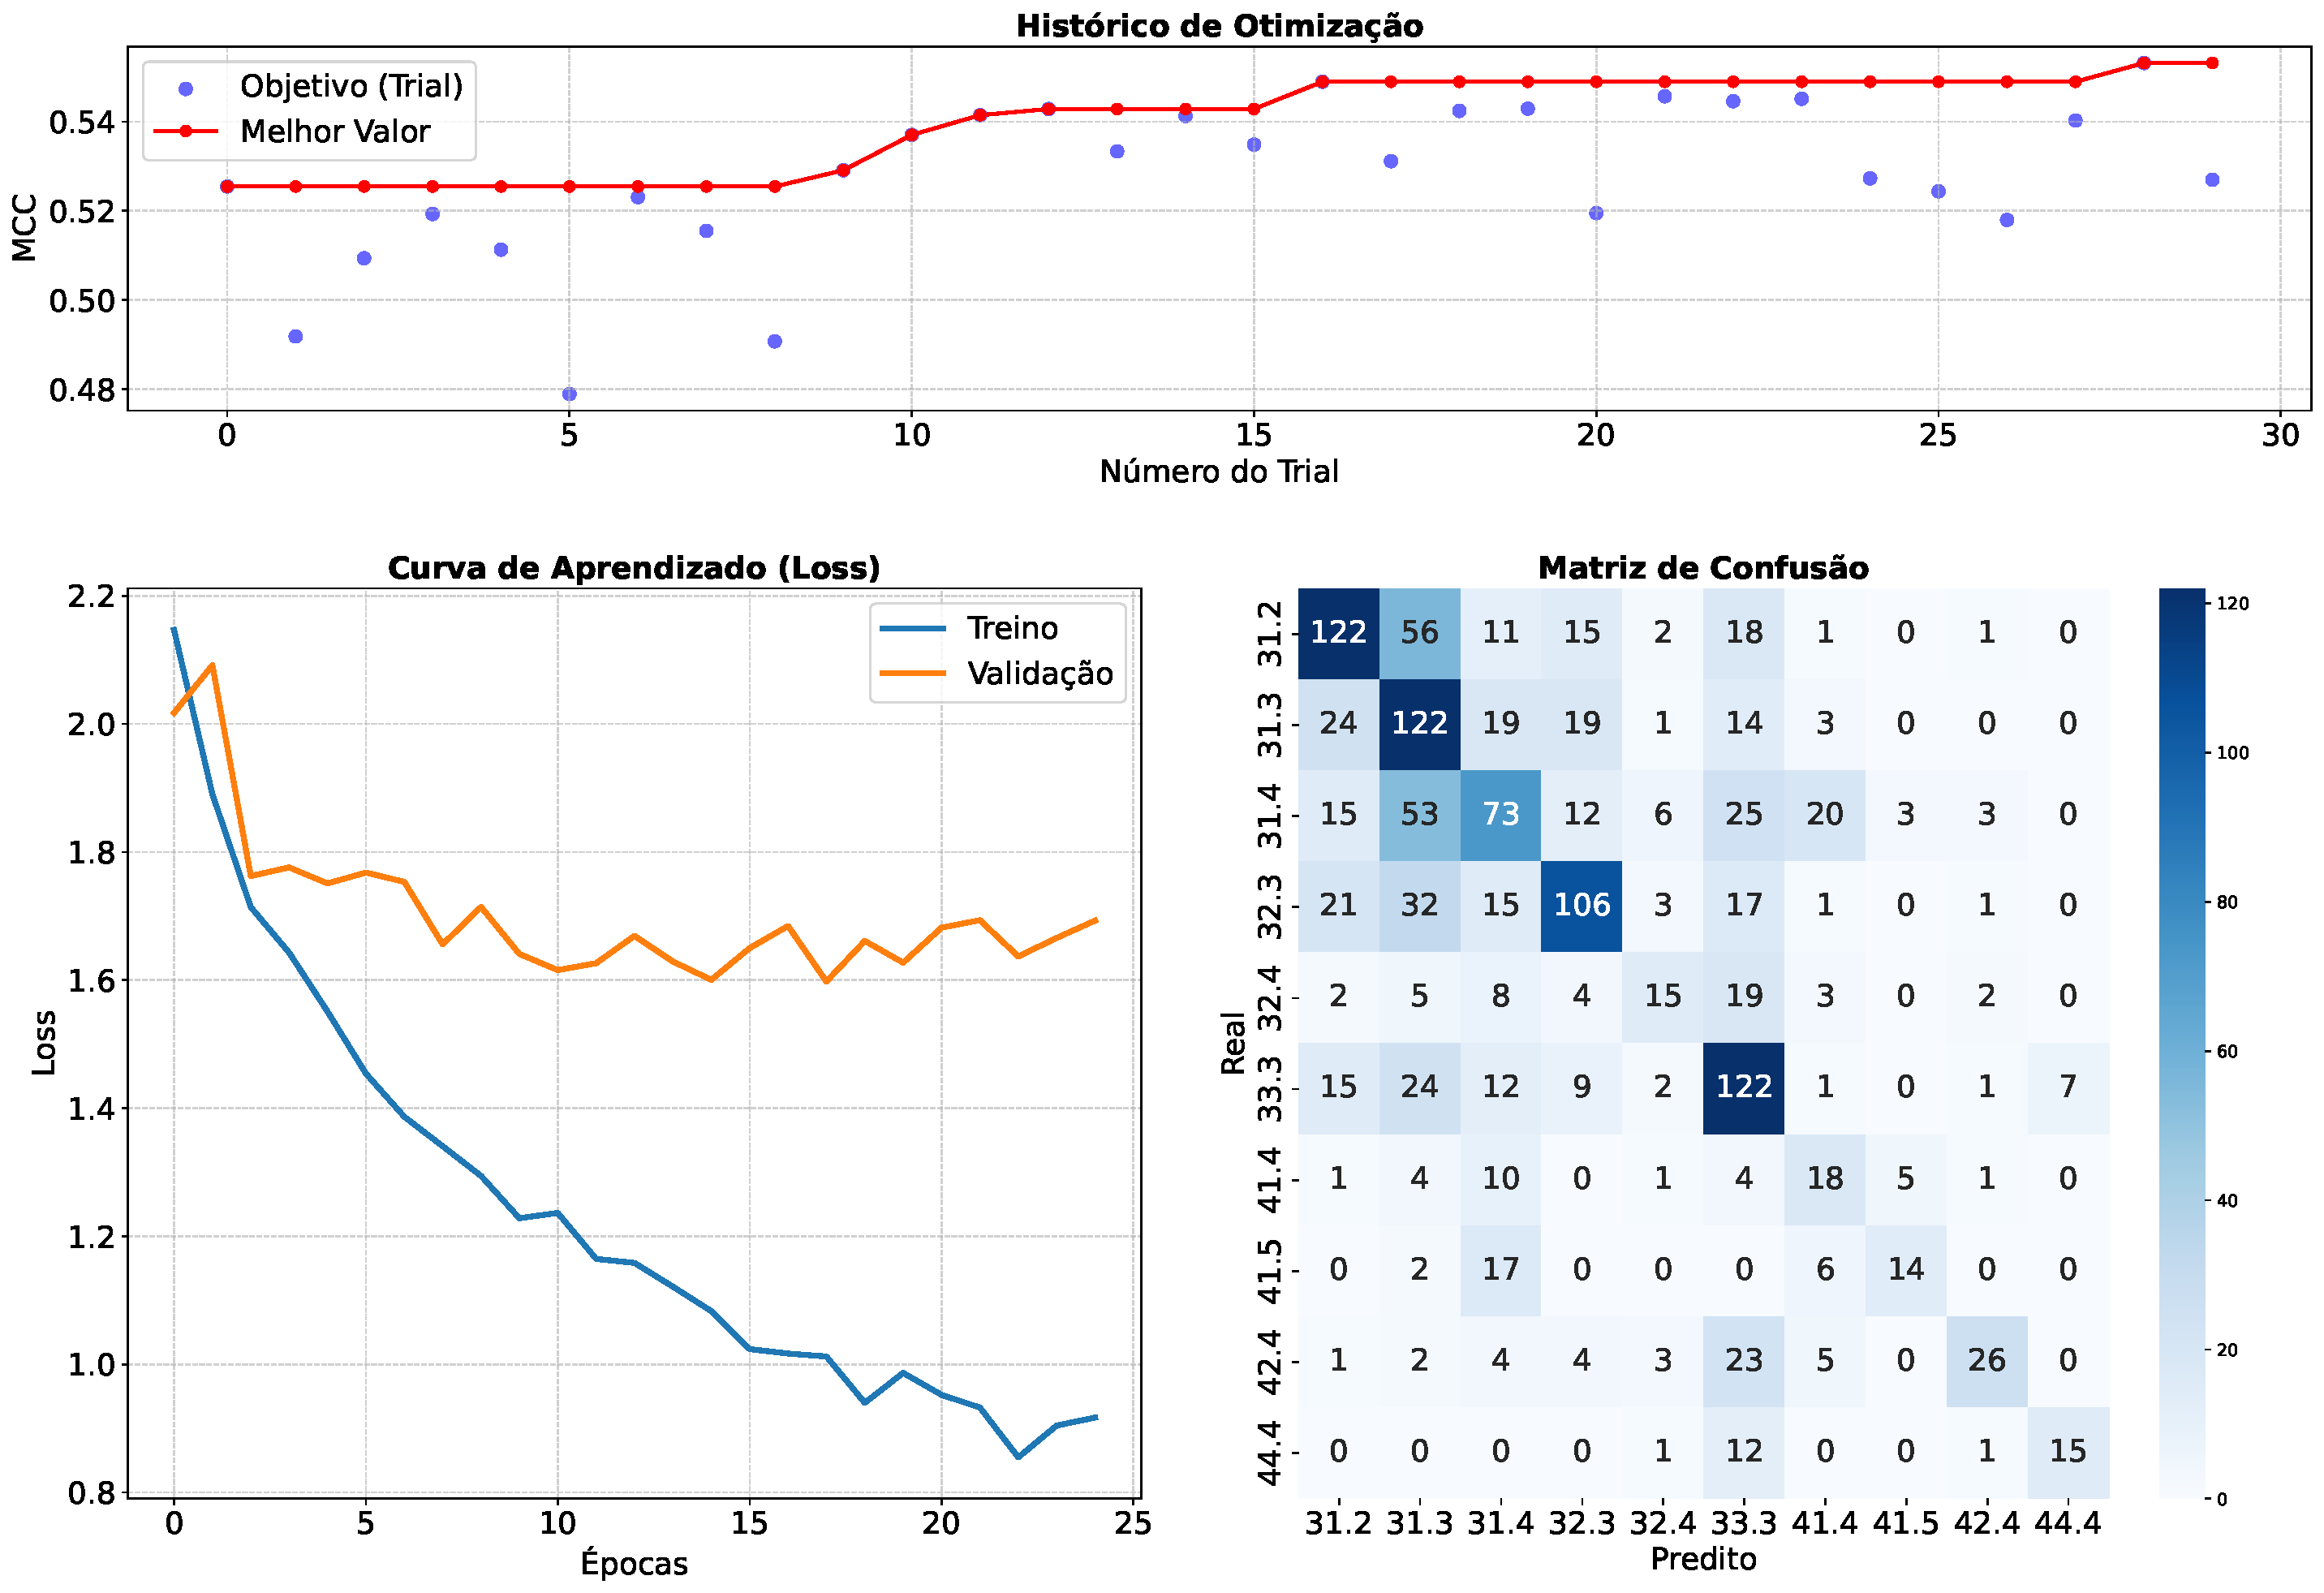
\includegraphics[width=0.85\textwidth]{tex/appendix/experiments/vit_v1_AB_opt_aug/dashboard_consolidado.pdf}
        \caption{Histórico de Otimização, Curvas de Aprendizado e Matriz de Confusão - vit\_v1\_AB\_opt\_aug}
    \end{figure}
\end{minipage}
\clearpage
